%
% 1. process this file with pdflatex
% 2. remind to process it twice otherwise cross-references will be wrong
%
\documentclass[a4paper,12pt]{article}
%
% This is to create hyperlinks for index, URLs and citations (now we can use the
% command \url{...} to create URL with hyperlink)
%
\usepackage{color}
\usepackage{listings}
\lstset{
    tabsize=2, % tab space width
    showstringspaces=false, % don't mark spaces in strings
    commentstyle=\color{green}, % comment color
    keywordstyle=\color{blue}, % keyword color
    stringstyle=\color{red} % string color
}
\usepackage[a4paper,colorlinks=true,urlcolor=blue,citecolor=blue,linkcolor=blue,bookmarks=false]{hyperref}
%
% This allows inclusion of pictures. Create figures with PowerPoint and then
% export them individually in PDF, PNG, JPEG, or GIF format (in order of
% preference)
%
\usepackage[pdftex]{graphicx}
\DeclareGraphicsExtensions{.pdf,.png,.jpg,.gif}
%
% phantom space (for abbreviations)
%
\usepackage{xspace}
%
% Definition of margins
%
\usepackage[top=2cm,bottom=2cm,left=2cm,right=2cm]{geometry}
%
% This is needed if you write the report in Italian
%
\usepackage[latin1]{inputenc}% IMPORTANTE! usare codifica ISO-8859-1 per le lettere accentate
%
% Paragraph skip and indent
%
\setlength\parskip{\medskipamount}
\setlength\parindent{0pt}
%
% Frequently used abbreviations.
% - example1: \ie this is an example
% - example2: the \ipsec protocol
%
\def\eg{e.g.\xspace}
\def\ie{i.e.\xspace}
\def\myfig#1{Fig.~#1\xspace}
\def\mytab#1{Tab.~#1\xspace}
\def\rfc#1{RFC-#1\xspace}% usage: \rfc{1422}
%
\begin{document}

\title{Security of Docker containers \\
{\normalsize Report for the Computer Security exam at the Politecnico di Torino}
} \author{Carmine D'Amico (239540) \\
{\normalsize tutor: Antonio Lioy} }
\date{? 2018}
\maketitle

\vfill

\rule{\textwidth}{1pt}

\tableofcontents

\rule{\textwidth}{1pt}

\vfill

\newpage

\section{Introduction}

\newpage

\section{Docker Overview}

In computer science, the term \textit{virtualisation} is referred to the
creation of virtual computational resources\cite{wikipedia_virtualization}.
These resources, normally supplied as hardware, are instead provided to the user
by the operating system through the creation of a new abstraction layer.
Operating systems, storage devices or network resources could all be
virtualised. Virtualisation can be obtained at different levels and using
different techniques. \par\textit{Virtual machines} have represented for many
years the state of the art of virtualisation, being used in both consumer and
enterprise contexts. In the last years a new technology, based on
\textit{containers}, has started to gain more attention specially thanks to its
advantages in terms of acceleration of the development cycle and possibility to
thicken applications on servers. \textit{Docker} is an open source container
technology became popular thanks to its simple interface, which allows to create
and manage containers in an easy way. 

\subsection{From Virtual Machines...}

With the term virtual machines it is often intended an \textit{hypervisor-based
virtualisation}, that is a type of virtualisation which acts at hardware level.
Virtual machines (VMs) are established on top of the host operating system,
providing applications with their dependencies, but also an entire guest OS and
a separate kernel. One or more virtual machines can be run on the same machine.
Hypervisors are distinguished in two different types, the one that works
directly on top of the host's hardware (\textit{bare metal hypervisor}) and the
one that is on top of the host's OS (\textit{hosted hypervisor})
(\myfig{\ref{fig:hypervisor_difference}}). \par Bare metal hypervisor provides
better performances, not having the overhead of the extra layer of the host's
operating system. It manages directly hardware and the guest's operating system.
On the contrary hosted hypervisor can be manged in an easier way running as a
normal computer program on the user's operating
system\cite{types_of_hypervisor}. \par As said before, the hypervisor needs to
run on the user's computer which is defined as \textit{host machine}, while each
virtual machines is called \textit{guest machine}. It is important to remember
this terminology because it will be used also in the following, referring to
containers. 

\begin{figure}[ht!]
  \centerline{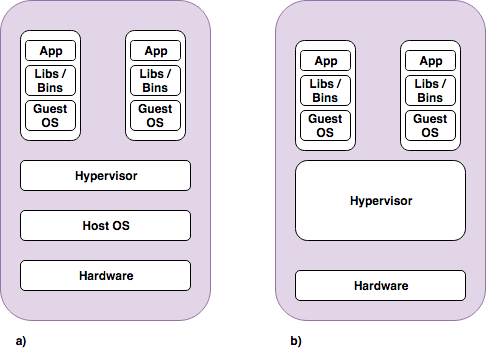
\includegraphics[width=0.7\textwidth]{difference_bare_metal_hosted_hypervisor.png}}
  \caption{Architectural differences between (a) hosted hypervisor and (b) bare metal hypervisor}
  \label{fig:hypervisor_difference}
  \end{figure}


\subsection{...To Containers}

\textit{Container-based virtualisation} represents another approach to
virtualisation, mainly spread in the last years. Compared to hypervisor-based
virtualisation it results lighter, using the host's kernel to run multiple
virtual environments. It virtualises at operating system level (it is also known
as \textit{OS-level virtualisation}) allowing other applications to run without
installing their own kernel on the host. Containers look like separated processes
that just share host's kernel and are more isolated from the host's
system (\myfig{\ref{fig:container_architecture}}). \par Resources are provided by
the host's OS together with the container engine. A container engine is the
technology in charge of create and manage containers. \textit{Docker} represents
one of the most important and most used container engine. A computer program
running inside a container can only see the resources allocated to that particular
container. On the same host there could be more than one container, each one
with its personal set of dedicated resources. Although it could be possible to
run more than one computer program inside the same container, it is always
suggested to run only one program per container, in order to separate areas of
concern. It is better to connect multiple containers using user-defined networks
and shared volumes. Containers are particularly appreciated inside multitenant
environments for their lightness and for their approach to host's resources
sharing, which increases average hardware use.\par There are many examples of
containerisation implementations, like \textit{Linux-VServer}, \textit{OpenVZ}
and \textit{LinuX Container (LXC)}. This last implementation will be better
described in the next section allowing to better understand the behaviour of
containers. 

\begin{figure}[ht!]
  \centerline{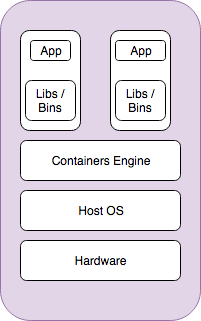
\includegraphics[width=0.3\textwidth]{container_architecture.png}}
  \caption{Architecture of a container-based virtualisation}
  \label{fig:container_architecture}
  \end{figure}

% figure of the OS virtualisation

\subsection{LXC}

\textit{LinuX Containers}, better known as LXC, are an OS-level virtualisation
technique created around 2008. They allow to run multiple isolated Linux
instances (the \textit{containers}), on top of a single \textit{LXC host}, which
shares its Linux kernel\cite{wikipedia_LXC}. Each container "sees" its own CPU,
memory, network interface, I/O, ecc... \par The isolation among containers is
obtained thanks to some Linux kernel's tools: namespace and cgroups. In the
following subsections these two components will be analysed, both for their
importance for containerisation and for the fact that they are also the basic
components in Docker.

\subsubsection{Kernel Namespace}

\textit{Namespaces} allow to create isolated environments, in which each process
that belongs to that particular environment can see global host's resources as
personal isolated resources. In other words they allow to create pool of
processes that think to be the only ones of the system. In this way groups of
processes, that are part of different namespaces, can see different set of
resources. Namespaces work by assigning to different resources the same name in
different namespaces. In the Linux kernel six different type of environments are
implemented\cite{red_hat_introduction_to_namespaces}:
  \begin{itemize}
    \item \textbf{Mount namespaces} isolate the set of file system mount points
    seen by a group of processes so that processes in different mount namespaces
    can have different views of the file system hierarchy. With mount
    namespaces, the mount() and umount() system calls cease to operate on a
    global set of mount points (visible to all processes) and instead perform
    operations that affect just the mount namespace associated with the
    container process. 
    \item \textbf{UTS namespaces} isolate two system identifiers (nodename and
    domainname) returned by the uname() system call. This allows each container
    to have its own hostname and NIS domain name which is useful for
    initialisation and configuration scripts based on these names. 
    \item \textbf{IPC namespaces} isolate certain inter-process communication
    (IPC) resources, such as System V IPC objects and POSIX message queues. This
    means that two containers can create shared memory segments and semaphores
    with the same name, but are not able to interact with other containers
    memory segments or shared memory. 
    \item \textbf{Network namespaces} provide isolation of network controllers,
    system resources associated with networking, firewall and routing tables.
    This allows container to use separate virtual network stack, loop-back device
    and process space. In this way it is possible to add virtual or real devices
    to the container assigning them their own IP Addresses and even full iptables
    rules. 
    \item \textbf{PID namespaces} allow processes in different containers to
    have the same PID, so each container can have its own init (PID1) process
    that manages various system initialisation tasks as well as containers life
    cycle. Also, each container has its unique \textit{\/proc} directory. From
    within a container only processes running inside the container can be
    monitored. The container is only aware of its native processes and can not
    "see" the processes running in different parts of the system. On the other
    hand, the host operating system is aware of processes running inside of the
    container, but assigns them different PID numbers.
  \end{itemize} 

\subsubsection{Cgroups}

\textit{Cgroups} are a kernel tool used to manage processes' resources. They
gather, track and limit processes' usage of resources. It is possible to create
and manage \textit{cgroups} using high level code, assigning PID to a specific
\textit{cgroup}. They represent the fundamental tool to obtain resource
isolation, playing an important role also for the CPU and I/O's scheduling. The
resources that can be limited by Cgroups
are\cite{red_hat_introduction_to_cgroups}:
\begin{itemize}
  \item \textbf{memory} - this subsystem sets limits on memory use by tasks in a
  cgroup and generates automatic reports on memory resources used by those
  tasks. 
  \item \textbf{CPU} - this subsystem uses the scheduler to provide cgroup tasks
  access to the CPU. 
  \item \textbf{CPUacct} - this subsystem generates automatic reports on CPU
  resources used by tasks in a cgroup. 
  \item \textbf{CPUset} - this subsystem assigns individual CPUs (on a multicore
  system) and memory nodes to tasks in a cgroup.
  \item \textbf{blkio} - this subsystem sets limits on input/output access to
  and from block devices such as physical drives (disk, solid state, or USB). 
  \item \textbf{net\_cls} - this subsystem tags network packets with a class
  identifier (classid) that allows the Linux traffic controller (tc) to identify
  packets originating from a particular cgroup task. 
  \item \textbf{net\_prio} - this subsystem provides a way to dynamically set
  the priority of network traffic per network interface. 
  \item \textbf{ns} - the namespace subsystem. 
  \item \textbf{devices} - this subsystem allows or denies access to devices by
  tasks in a cgroup. 
  \item \textbf{freezer} - this subsystem suspends or resumes tasks in a cgroup.
  \item \textbf{perf\_event} - this subsystem identifies cgroup membership of
  tasks and can be used for performance analysis. 
\end{itemize}   

\subsection{Docker}

As today, \textit{Docker} represents the most used computer program for
operating-system-level virtualisation (containerisation). It is developed by
\textit{Docker, Inc}\cite{docker_official_site} and it was introduced during the
2013's PyCon conference. During its presentation, \par\textit{Docker} was
announced as the future of Linux Containers\cite{docker_pycon_presentation},
indeed from its first releases it reiterated many concepts from them, such as
\textit{Namespaces} and \textit{Cgroups}, but providing a simpler user
experience and a complete ecosystem to create and manage containers.\par
Docker's success is mainly addressable to its portability and lightweight
nature which allow to create high density environments. It is the ideal software
in scenarios where continuous integration and continuous delivery (CI/CD) are
required, allowing developers to not only build their code, but also test their
code in any environment type and as often as possible to catch bugs early in the
applications development life cycle \cite{docker_ci_cd}. 

\subsubsection{History}

\textit{Docker} was born as an inside project within \textit{dotCloud}, a
platform-as-a-service (PaaS) company, later renamed to \textit{Docker, Inc}.
Solomon Hyckes\cite{solomon_hyckes_wiki} was the leader of the project, that was
at first developed with other \textit{dotCloud}'s engineers, like Andrea
Luzzardi and Francois-Xavier Bourlet. The project went public, as said before,
during 2013's PyCon conference and it was released as open source software
during the same year. Always during 2013, \textit{Docker} distanced itself from
Linux Containers, replacing them with a new execution environment (starting from
version 0.9), \textit{libcontainer}.\par \textit{Docker} represented a turning
point in the IT industry, as it can be proved by looking ad its adoption. The
following is a list of the milestones achieved by the program, from
Wikipedia\cite{docker_history_wiki}:
\begin{itemize}
  \item On September 19, 2013, Red Hat and Docker announced a collaboration
  around Fedora, Red Hat Enterprise Linux, and OpenShift.
  \item In November 2014 Docker container services were announced for the Amazon
  Elastic Compute Cloud (EC2).
  \item On November 10, 2014, Docker announced a partnership with
  Stratoscale.
  \item On December 4, 2014, IBM announced a strategic partnership with Docker
  that enables Docker to integrate more closely with the IBM Cloud.
  \item On June 22, 2015, Docker and several other companies announced that they
  are working on a new vendor and operating-system-independent standard for
  software containers.
  \item As of October 24, 2015, the project had over 25,600 GitHub stars (making
  it the 20th most-starred GitHub project), over 6,800 forks, and nearly 1,100
  contributors.
  \item A May 2016 analysis showed the following organisations as main
  contributors to Docker: The Docker team, Cisco, Google, Huawei, IBM,
  Microsoft, and Red Hat.
  \item On October 4, 2016, Solomon Hykes announced InfraKit as a new
  self-healing container infrastructure effort for Docker container
  environments.
  \item A January 2017 analysis of LinkedIn profile mentions showed Docker
  presence grew by 160\% in 2016.[30] The software has been downloaded more than
  13 billion times as of 2017.

\end{itemize}   

\subsubsection{Docker's Architecture}

\textit{Docker} follows a client-server architecture where three main components
can be distinguished\cite{docker_architecture}
(\myfig{\ref{fig:docker-architecture}}):
\begin{itemize}
  \item The server, which is a daemon process (called \textbf{dockerd}) running
  on the host's machine. It is in charge of create and manage Docker's objects.
  \item A set of interfaces conformed to REST architectural style, that enable
  programs to communicate with the server, sending instructions.
  \item A command line interface (CLI) client, that allows the user to interact
  with Docker using the REST API through their terminal. 
\end{itemize}   

\begin{figure}[ht!]
  \centerline{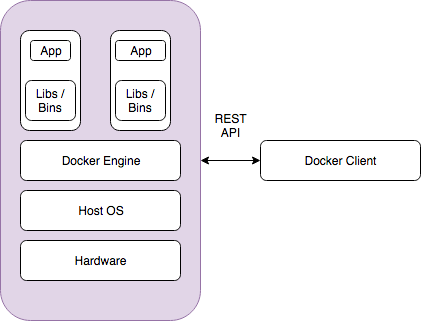
\includegraphics[width=0.6\textwidth]{docker_architecture.png}}
  \caption{Docker's architecture}
  \label{fig:docker-architecture}
  \end{figure}

\subsubsection{Docker's Components}
\label{sec:docker_object}

Docker's workflow includes the interaction with many special purpose components
created and managed by \textbf{containerd}:
\begin{itemize}
  \item \textbf{IMAGES} are the basic components involved in the creation of a
  Docker's container, they include all the instructions that the daemon has to
  follow in order to run a container. An image can be created from scratch or it
  can be based on already existing images (for example on the image of
  \textit{nginx} if we want to create a web server) where other needed
  components are installed. \par A \textit{Dockerfile} is a special file that
  follows a very simple syntax, which includes all the steps that must be
  followed in order to create an image. Each instruction represents a layer in
  the image. When a new layer is inserted (modifying the \textit{Dockerfile})
  and a container is rebuilt, only the new layer is rebuilt, speeding up the
  deployment's process. An image is built from a Dockerfile using the
  \textit{docker build} command. \par Another way to create an image is to run
  an already existing container, perform all the modifications needed and at the
  end save the status achieved as a new image with the \textit{docker commit}
  command.\par Docker images are stored inside registries which can be private
  or public. The two most famous public registries are \textit{Docker Cloud} and
  \textit{Docker Hub}, the latter is the default one visited by Docker for
  searching images. Developers can build their own images and upload them to the
  Docker Hub, or they can just download already existing images from it.
  Developers' images on Docker Hub are by default public, only the paid accounts
  can upload private images. These images take a standard name, that has the
  form "developer/repository". \textit{Docker, Inc.} provides some official
  images, called simply "repository".  
  \item \textbf{CONTAINERS} represent the running instances of images. The
  relationship between images and containers could be compared to the
  relationship between classes and objects in an object-oriented programming
  language like Java. A container can be connected to the network or to a
  storage and it can be defined by its image or by the configurations indicated
  starting it. A container can be launched using the \textit{docker run}
  command.\par When a container is started Docker searches locally for all the
  needed images (downloading them from online public registries if necessary),
  then a read/write file system is allocated, where the container can create or
  modifies file or directories.  By default a container can be connected to the
  external network using the host's connection. When a container is stopped  any
  changes to its state that are not stored in persistent storage disappear.
  \item \textbf{SERVICES} are supported from version 1.12 of Docker. Like in a
  distributed system, services represent the different pieces of an application.
  In particular in the context of Docker a service is just a running container
  in which it is defined the way that its image will be executed. Through
  services indeed a user could configure the port which a container will use,
  the number of replicas that will run of such container to better scale an
  application, etc... \par The services that will run on a host can be
  configured by a special Docker file: \textit{docker-compose.yml}. This file
  contains all the instructions that must be followed to run our application's
  services. For each service indicated it specifies where to pull the
  correspondent Docker image, the port mapping between the container and the
  host, the load-balanced overlay network that will be used and all the
  information needed to deploy such service (the number of replicas, the amount
  of resources needed, the restart policy, etc...).
  \item \textbf{SWARMS} are cluster composed by machines that are running
  Docker. A \textit{swarm manager} is a machine belonging to the cluster and in
  charge of executing the commands received. A user continues to run Docker
  commands normally as described before, the difference is that such commands
  are executed by the swarm manager, which decides how to run these commands
  (for example filling the host with less running containers or assigning to
  each host one instance of the specified container). In a cluster there could
  be more than one swarm manager. \textit{Workers} are machines belonging to the
  swarm, but without the same privileges of a swarm managers. They just provide
  more computational capacity to the cluster. In general all the machines inside
  a Docker swarm are referred as \textit{nodes}.
\end{itemize}

\subsubsection{Common Usage Of Docker}

As stated in the previous paragraphs, Docker's success is mainly attributable to
its simplicity of use and to its "lightness". Such characteristics have
increased its adoption among developers and organisations. John Willis, a
Technical Evangelist at Docker, during an interview for the IBM Infrastructure
Blog stated\cite{ibm_interview_john_willis} that the most common use cases for
Docker are mainly three:
\begin{itemize}
  \item \textit{Integration test}: With virtual machines running integration
  test could take also days. The virtual machines should be configured and
  installed, then after the tests they should also be rebase back to their
  original state. On the contrary with Docker the configuration and the
  execution of a containers takes less time and also rebase could be done in few
  seconds.
  \item \textit{Immutable delivery model}: With Docker when a developer needs to
  commit its code he can just commit a Docker image. In such a way the software
  tested on his own computer will be the same identical software which will run
  in production. This principle allows to speed up the deployment process, not
  requiring further configurations to run the software on the production hosts.
  \item \textit{Container as service}: Docker allows to build up a collection of
  pre-built binaries (Docker images) that can be shared, for example pushing
  them into the Docker Hub. In such a way an organisation can speed up its
  production and also increase its set of used tools, not needing to set up its
  own tools but just to pull new images.
  
\end{itemize}


\newpage

\section{Docker's Security Threats}
 
In this section I analyse the most important security threats for a Docker
system. For each possible threat I describe its characteristics and how it could
be possible to take advantage of it. I also provide a practical example of an
attack which exploits the vulnerability described, exception made for those
threats that are more generic, not regarding specifically Docker containers.
\par In the next section I will start from these security threats in order to
define the best practice to follow using Docker.

\subsection{Analysis Of Docker Security Threats}

In order to list the main security threats that afflict a Docker system, I
started from a possible definition of the attack surface for the Docker
containers. I have analysed a series of studies present in literature, from
Yasrab's paper "Mitigation Docker Security
Issues"\cite{mitigating_docker_security_issues_yasrab} to  "To Docker or Not to
Docker: A Security Perspective" written by Combe, Martin and Di
Pietro\cite{to_docker_or_not_to_docker}, through Sysdig's list of the well known
vulnerabilities of Docker\cite{sysdig_docker_vulnerabilities}. Finally, I have
divided the Docker attack surface in five macro areas:
\begin{itemize}
  \item \textit{Isolation}: The most important difference between a normal
  process running on a host and a Docker container is the degree of isolation of
  the latter. As seen in the previous section, Docker uses different Linux
  kernel features to achieve an optimal isolation. However, such tools must be
  well configured, because it is possible that their default behaviour leads to
  \textit{denial-of-service attacks}, \textit{container breakouts} or
  \textit{ARP spoofing attacks}.
  \item \textit{Host Hardening}: Docker containers share the kernel with the
  host making them lighter than a virtual machine. Such characteristic
  increases the importance of the kernel security, cause both the containers and
  the host depend on it. \textit{Kernel exploits}, for example, can lead to
  malfunctions of both the host and the containers. 
  \item \textit{Network Security}: Docker relies completely on the network for
  the distribution of images. If some attacker obtains to \textit{poison the
  images} that a container is downloading, he can damage the entire system.
  \item \textit{Erroneous Configurations}: Docker has made of its simplicity of
  use its most important feature. However some precautions must be taken
  configuring a Docker system. For example an \textit{erroneous management of
  the secrets} can bring to an impairment of the system. As well as the use of
  \textit{outdated Docker images}, can lead to have bugs in the system easily
  exploitable by an attacker.
  \item \textit{Running Container}: Inside a Docker container there is anyway
  our running program. All the bugs and vulnerabilities that afflict our program
  can be used by an attacker to hit our system. For this reason, to cover all the
  attack vectors of our Docker containers, we should also \textit{monitor the
  runtime activities of our containers}.
\end{itemize}
From these macro areas, I have extracted eight security threats for Docker
containers, analysing them in the following paragraphs.
 
\subsubsection{Kernel Exploits}

One of the main advantages of container-based virtualisation, so of Docker,
is that the host shares its kernel with all the running containers. In this way
this kind of virtualisation results lighter than an hypervisor-based one,
avoiding the overhead of installing the guest's kernel. As we will see this is
on the one hand a big advantage in terms of speed and efficiency, but on the
other hand it represents a big threat for the security of the system. The host's
kernel, indeed, handles all the containers' operations, so in case of a
\textit{kernel-level exploit} all the containers that are running on the system
are at risk of being compromised.\par Kernel exploits can be done by an attacker
who takes advantages of a bug or a vulnerability of the kernel. In this way he
can run his software in kernel mode, manipulating processes' privileges and
bringing him to take control of the system. If such exploit is performed inside
a container, it has consequences also on the host OS. In particular if the
attack allows the attacker to execute his code, this execution will happen on
the host OS, not inside the container; in the same way if the attack allows to
read arbitrary memory, so the attacker could read and write memory parts that
belong to other containers.\par Kernel exploits are also a security threat in
the context of an hypervisor-based virtualisation, but in that case the attack
would result more complicated. Indeed the attacker should be able to exploit the
VM's kernel, the hypervisor and the host's kernel. While on a container-based
virtualisation it is sufficient to exploit the only host's kernel.

\bigbreak\textbf{Practical Example}\bigbreak 

In literature there are many examples of kernel exploits used to obtain control
over an entire system. In this section I will focus on \textit{Dirty COW}, an
attack that takes advantage of a privilege-related vulnerability in order to
allow the attacker to gain high privileges on the system. The official reference
to this bug is CVE-2016-5195.\par It exploits a race condition inside the Linux
kernel's memory subsystem that handles the copy-on-write (COW) mechanism, in
this way an unprivileged user could gain write access to a read-only memory
part\cite{red_hat_dirtycow}.\par In order to obtain this exploit, we must create
a loop involving two threads:
\begin{itemize}
  \item one thread tries to access inside a read-only memory location to
  write, creating in this way a modified copy inside the process's memory
  \item another thread, calls the syscall
  \textit{madvise()}\cite{madvise_description} with the MADV\_DONTNEED parameter
  (such parameter indicates that is not to be expected to access the memory
  location in question) for the newly allocated memory
  \end{itemize}
The simultaneous execution of these two threads in a loop could bring the
kernel to point to the modified copy of a file in memory that should instead be
read-only\cite{dirtycow_how_it_worrks}.

\subsubsection{Denial-of-service}

As we have seen for kernel exploits, the fact that all the containers running on
a host share the same kernel can be positive and negative at the same time. All
the containers, indeed, share also the same resources and if the access to them
is not limited in some way one container could require a huge amount just for
it, bringing the host and the other containers to starvation. This type of
attack is known as \textit{denial-of-service(DoS)}.\par Denial-of-service
attacks are very well-known attacks in literature, especially in multi-tenant
systems, that are the ones where Docker is mostly used.  The aim of the attack
is to make a system or a network resource unavailable. It is typically
accomplished by flooding the targeted machine or resource with superfluous
requests in an attempt to overload systems and prevent some or all legitimate
requests from being fulfilled\cite{dos_wikipedia}. An attack of this genre,
conducted against a Docker container, brings to unavailability not only the
container itself, but also the host where it is virtualised together with all
the other system's containers.\par On a virtual machine this type of attack is
also possible, but it is more difficult to be completed. This is due to the fact
that the hypervisor is configured to restrict its use of resources. For a
container, instead, resources management is defined at application layer.\par
In the previous section we have seen how Docker has inherited Cgroups from LXC
to allocate containers' resources. However, as described on Docker's
documentation\cite{resource_on_docker}, this kernel tool is not enabled by
default, so a container can use as much of a given resource as the host's kernel
scheduler allows. We will see in the next section how to configure Docker to
work with Cgroups, managing resources for containers. 

%\bigbreak\textbf{Practical Example}\bigbreak 

\subsubsection{Container Breakout}

If a user inside a Docker container bypasses all the isolation checks,
"escaping" from the container, it would have direct access to the host and to
all the other containers in the system. This situation can be achieved using an
exploit or a not correct configuration of the Docker environment. Such type of
attack is known as \textit{container breakout}.\par This type of vulnerability,
according to Docker website\cite{docker_blog_about_container_breakout}, was
fixed in Docker 1.0, nevertheless a not trusted program running with root
privileges inside a Docker container could still represent a source of risk.
\par Container breakout was mostly possible in situations where privileges
inside a container were not properly configured. By default, users are not
namespaced, so any process that breaks out of the container will have the same
privileges on the host as it did in the container. A root user in a container
will also be root on the host. Moreover, in the earliest versions of the Docker
engine, some specific kernel capabilities were dropped, but still leaving some
important ones granted. From Docker 1.0, instead, a different approach was
taken: all the capabilities were dropped, giving the user the possibility to
decide which one to allow. De facto this newly approach transformed the use of
capabilities from a blacklist to a white-list.

\bigbreak\textbf{Practical Example}\bigbreak 

One of the most famous container breakout exploit is 2014's
\textit{Shocker}\cite{shocker}. We will analyse such attack, with the aim to
demonstrates how a Docker container could access some privileged file-system
data. As said before, this kind of vulnerability was fixed with Docker 1.0, but
it could still be interesting to understand how this type of attack
worked\cite{shocker_how_it_works}.\par Shocker takes advantage of the
\textit{CAP\_DAC\_READ\_SEARCH} capability, that was granted by default to a
superuser inside a Docker container. This capability is the one which allows to
use the system call \textit{open\_by\_handle\_at()}, conceding to access a file
on a mounted file-system through a file\_handle structure. A file\_handle is
quite different than a file descriptor, because it can be generated inside a
process using \textit{name\_to\_handle\_at()} and then recalled by another
process with \textit{open\_by\_handle\_at()} (while a file descriptor can't be
properly passed between different processes). In this way if a process has an
handle opened for a host's file or a different container's file and our
container has not the privileges to access it, we can still call
\textit{open\_by\_handle\_at()} on the opened handle.

\subsubsection{Poisoned Images}

As said in \ref{sec:docker_object}, Docker images represent one of the most
fundamental building blocks for a container. If an attacker could obtain to make
his images to run, the host and all its containers are seriously at risk. \par
Container images are claimed to be downloaded and verified by default by the
system, thanks to the presence of a signed manifest inside the image. In such
mechanism however Docker does not verify the image's checksum from the manifest.
In this way an attacker could provide his \textit{poisoned images} with some virus,
together with a signed manifest, tricking Docker verification and leading to
many vulnerabilities the user's system. \par Jonathan Rudenberg explained, in a
post\cite{docker_image_insecurity} on his blog, how the process of downloading a
Docker image from the Docker Hub is extremely insecure. Such images are
downloaded from an HTTPS server and then they immediately go through a
processing pipeline inside the Docker daemon: \bigbreak\centerline{decompress
$\,\to\,$ tarsum $\,\to\,$ unpack}\bigbreak This pipeline, even if it is
functional, is insecure. The reason lies in the fact that the not trusted input
is processed before its verification. 

\bigbreak\textbf{Practical Example}\bigbreak 

CVE-2014-9357\cite{CVE-2014-9357} is a known vulnerability that allowed remote
attackers to execute arbitrary code with root privileges via a crafted image or
build in a Dockerfile in an LZMA (.xz) archive, related to the chroot for
archive extraction.\par This vulnerability exploited the way the Docker service
unpacked images or builds after a "docker pull". In such a way an attacker could
use this flaw to provide a malicious image or build that, when unpacked, would
escalate their privileges on the system.

\subsubsection{Static Images' Threats}

The importance of images in Docker ecosystem makes it of primary importance to
attest their security. On the one hand we have seen how images could be
\textit{poisoned} by an attacker, on the other hand even if no attacker tries to
manipulate our images it doesn't mean that our images are safe. It is important
to make sure that the images at the base of our running containers are updated,
not containing any known vulnerabilities. An outdated image can be affected by a
series of security threats that were already fixed in an updated version of the
same image. \par A study by Gummaraju, Desikan, and Turner at BanyanOps
demonstrated how about more than the 30\% of the official repositories present
on Docker Hub are affected by a variety of security threats, such as
\textit{heartbleed}, \textit{shellshock}, \textit{poodle}, etc... These numbers
grow up to the 40\% taking in consideration also the images loaded by
users\cite{gummaraju_desikan_turner}. 

\subsubsection{Management Of Secrets}

Docker containers are very used in the development of microservices. A
microservice architecture is very different than a monolithic one, specially in
the deployment phase: a monolithic architecture is often just configured,
launched and then it runs for a long period of time (which could even last
years); microservices are continuously created and destroyed. In both cases,
sensitive information are needed, like API keys, database passwords, SSL/TLS
keys, SSH keys, etc... Compromising these information would compromise the
entire system. \par In a monolithic architecture the management of these
information's is non trivial, having them stored in the system permanently with
mechanisms for their renovation, like the "Privileged Accounts
Managers"\cite{privileged_accounts_managers}. Despite these solutions have been
used and tested for years in the context of monolithic service, they can't be
applied to microservices based on containers. The two main concerns for the
management of secrets inside Docker containers
are\cite{secret_management_concerns_docker}:
\begin{itemize}
  \item Docker images have an immutable nature, this means that they are created
  once and then deployed in many different environments. Their nature is
  strongly in contrast with the idea of saving secrets directly inside them.  
  \item Requesting such secrets at runtime imply performing a prior
  authentication procedure, but this procedure is difficult to be implemented
  without storing some secrets for the authentications itself.
\end{itemize}
\par In the case of Docker, a security breach inside a single container could
lead to the breakdown of all the other containers running on the same host. For
this reason \textit{management of secrets} should be seen as an important threat
for Docker containers' security.

\bigbreak\textbf{Practical Example}\bigbreak 

One example of how a bad management of secrets could be fatal for an agency
comes from IBM. In 2017 a privilege escalation vulnerability was found inside
IBM Data Science Experience, a data analytics
product\cite{ibm_data_science_experience}. Such vulnerability was due to a wrong
configuration of the Docker containers that were running the service. IBM's
engineers left inside the containers Docker TLS keys, leaving root access across
the whole computer cluster and read/write access many terabytes of sensible
customer data. \par As stated by the report of the
vulnerability\cite{ibm_data_sciene_report}, an exploit of such threat was also
quite easy, needing only an access to to Internet and a web browser:
\begin{itemize}
  \item The attacker should just enter the service's web environment, accessing
  to its command line
  \item He should download and extract the Docker binary of the service, using
  the following commands: 
  \begin{lstlisting}[language=bash,breaklines]
    system("wget https://test.docker.com/builds/Linux/x86_64/docker-1.13.1-rc1.tgz")
    system("wget https://test.docker.com/builds/Linux/x86_64/docker-1.13.1-rc1.tgz")
  \end{lstlisting}
  \item Use the downloaded Docker binary with the existing certificates to
  achieve root access to the host mounted volume:
  \begin{lstlisting}[language=bash,breaklines]
    system("DOCKER_API_VERSION=1.22 ./docker/docker -H 172.17.0.1 \
              --tlscacert /certs/ca.pem --tlscert /certs/cert.pem \
              --tlskey /certs/key.pem \
              run -v /:/host debian cat /host/etc/shadow")
  \end{lstlisting}
\end{itemize} 

\subsubsection{ARP Spoofing}

Inside an host, all the containers, if not properly configured, can communicate
with each other through their network interfaces. Docker uses namespaces to
create an independent network stack for each container, giving them their own
own IP addresses, IP tables, etc... By default Docker provides connectivity
between the containers creating a Virtual Ethernet Bridge, named
\textit{docker0}. At container creation time, Docker creates and connect a new
network interface with a unique name to the bridge. Such interface is also
connected to the \textit{eth0} interface of the
container(\myfig{\ref{fig:docker_network_model}}). This type of configuration is
vulnerable to \textit{ARP spoofing} attacks, since the bridge forwards all of
its incoming packets without any filtering. \par An ARP spoofing attack is a
very well known attack in literature. It takes advantage of the ARP protocol,
which doesn't provide a basic method to authenticate ARP messages. In order to
perform such type of attack, the attacker must be connected directly to the
target LAN with his machine or running a compromised host that belongs to the
network. In the case of Docker, such conditions is satisfied if the attacker
manages to compromises a container running on a host: in this way he would have
access to the local network between all the containers running on the host. The
main goal of this type of attack is to divert traffic directed to a container to
the compromised container controlled by the attacker.   
\begin{figure}[ht!]
  \centerline{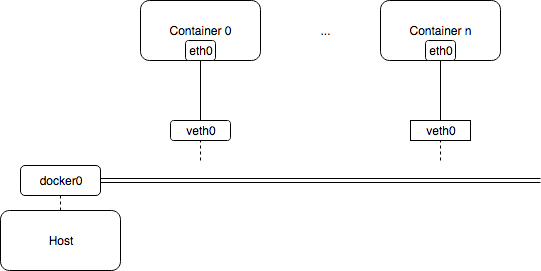
\includegraphics[width=0.7\textwidth]{docker-network-model.png}}
  \caption{Docker default network model}
  \label{fig:docker_network_model}
  \end{figure}

\bigbreak\textbf{Practical Example}\bigbreak 

A practical example of this type of attack can be reproduced inside a
containerised environment just running a Docker container with \textit{dSniff}
installed. Dsniff is a set of password sniffing and network traffic analysis
tools, which contains among others also \textit{arspoof}, a tool used
specifically to perform ARP spoofing attack\cite{wiki_dsniff}. \par Such type of
experiment is described by Philipp Bogaerts in one of his blog post
\cite{bogaerts_arpspoof}. He shows how it is simple to perform an ARP spoofing
attack running three containers on the same host, without changing the default
network configuration:
\begin{itemize}
  \item Two containers are created just from the Busybox base image, running the
  "ifconfig" command on each in order to read their IP address. We will call
  these two containers just \textit{container\_0} and \textit{container\_1}.
  \item One container, which will be the one that performs the attack, is created
  starting from the Debian base image, to which it is installed only dSniff. 
\end{itemize}
One of the first two containers ping the other, while the attacker's container
performs the attack using arspoof:
\begin{lstlisting}[language=bash,breaklines]
  arpspoof -i eth0  -t ip_container0 ip_container1 &
  arpspoof -i eth0  -t ip_container1 ip_container0 &
\end{lstlisting}
In such a way all the traffic generated between the first two containers will
pass through the attacker's container.

\subsubsection{Dynamic Aspects of Docker Security}

All the threats analysed in the former sections regard the launch-time of
containers. Kernel exploits, denial-of-service, container breakouts, etc... are
all security threats that can be faced before running our containers. We can
refer to these as \textit{static aspects} of Docker security. Such threats, as
we will see in the next chapter, can all be mitigated following some precautions
during the creation of the images that we will run, using special configurations
and ad-hoc policies or tools.\par However container's attack surface is not
limited to such aspects, we must also consider:
\begin{itemize}
  \item All the possible vulnerabilities of the application that we want to run
  inside a container, that can be exploited by an attacker
  \item All the attacks that can be performed on a vulnerability already
  discovered but not yet patched (these attacks are also known as zero-day
  attacks)
\end{itemize}
Such attacks can not be avoided at launch-time, but they must be mitigated at
runtime, monitoring containers' activity . We can refer to them as
\textit{dynamic aspects} of Docker Security. 

%\subsubsection{Summary}

%All the attacks listed above are summarised in Tab. 1. In the next section I
%will provide a list of best practices to follow using Docker in order to prevent
%such threats. For this reason in the following table each attack is associated
%with a code, that will be reused in the next section to associate to each best
%practice the attack that it prevents.

%\begin{table}[ht]
%  \begin{tabular}{ | l | l | p{5cm} |}
%  \hline
%  Code & Threat & Practical Example \\ \hline
%  T1 & Kernel Exploit & test \\ \hline
%  T1 & 11C & test \\ \hline
%  T1 & 11C & test \\ \hline
%  T1 & 11C & test \\ \hline
%  T1 & 11C & test \\ \hline
%  T1 & 11C & test \\ \hline
%  T1 & 11C & test \\ \hline
%  T1 & 11C & test \\ 
%  \hline
%  \end{tabular}
%  \caption{Lorem Ipsum}
%  \label{table:docker_threats}
%\end{table}


\newpage

\section{Best Practices For Docker Deployment}

\newpage

\section{Experimental Evaluation}

\newpage

\section{Conclusions}

\newpage

\begin{thebibliography}{99}

\bibitem{wikipedia_virtualization}
"Virtualisation" Wikipedia Page,\\ \url{https://en.wikipedia.org/wiki/Virtualization}

\bibitem{types_of_hypervisor}
Thanh Bui,
``Analysis of Docker Security'',
January 2015

\bibitem{wikipedia_LXC}
"LXC" Wikipedia Page,\\ \url{https://en.wikipedia.org/wiki/LXC}

\bibitem{red_hat_introduction_to_namespaces}
Introduction to Linux Containers,\\ \url{https://access.redhat.com/documentation/en-us/red_hat_enterprise_linux_atomic_host/7/html/overview_of_containers_in_red_hat_systems/introduction_to_linux_containers}
  
\bibitem{red_hat_introduction_to_cgroups}
Introduction to Control Groups (Cgroups),\\ \url{https://access.redhat.com/documentation/en-us/red_hat_enterprise_linux/6/html/resource_management_guide/ch01}

\bibitem{docker_official_site}
Docker official site, \url{https://www.docker.com/}

\bibitem{docker_pycon_presentation}
The future of Linux Containers, PyCon 2013\\ \url{https://www.youtube.com/watch?v=wW9CAH9nSLs}

\bibitem{docker_ci_cd}
CI\/CD in Docker,\\ \url{https://www.docker.com/use-cases/cicd}

\bibitem{solomon_hyckes_wiki}
"Solomon Hikes" Wikipedia Page,\\ \url{https://en.wikipedia.org/wiki/Solomon_Hykes}

\bibitem{docker_history_wiki}
"Docker History" Wikipedia Page,\\ \url{https://en.wikipedia.org/wiki/Docker_(software)#History}

\bibitem{docker_architecture}
Docker architecture,\\ \url{https://docs.docker.com/engine/docker-overview/#docker-architecture}

\bibitem{docker_objects}
Docker objects,\\ \url{https://docs.docker.com/engine/docker-overview/#docker-objects}

\bibitem{ibm_interview_john_willis}
The most common use cases of Docker containers and organisations, \\ \url{https://www.ibm.com/blogs/systems/the-most-common-use-cases-of-docker-containers-and-organizations/}

\bibitem{mitigating_docker_security_issues_yasrab}
Robail Yasrab,
``Mitigating Docker Security Issues'',
April 2018

\bibitem{sysdig_docker_vulnerabilities}
Seven Docker security vulnerabilities and threats,\\ \url{https://sysdig.com/blog/7-docker-security-vulnerabilities/}

\bibitem{red_hat_dirtycow}
CVE-2016-5195,\\ \url{https://access.redhat.com/security/cve/cve-2016-5195} 

\bibitem{madvise_description}
MADVISE (2), \\ \url{http://man7.org/linux/man-pages/man2/madvise.2.html}

\bibitem{dirtycow_how_it_worrks}
Demonstrating the Dirty Cow exploit, \\ \url{https://01.org/developerjourney/recipe/demonstrating-dirty-cow-exploit}

\bibitem{dos_wikipedia}
Denial-of-service attack, \\
\url{https://en.wikipedia.org/wiki/Denial-of-service_attack}

\bibitem{resource_on_docker} 
Limit a container's resources, \\ \url{https://docs.docker.com/config/containers/resource_constraints/}

\bibitem{docker_blog_about_container_breakout}
Docker Container Breakout Proof-of-Concept Exploit, \\ \url{https://blog.docker.com/2014/06/docker-container-breakout-proof-of-concept-exploit/}

\bibitem{shocker}
Shocker, \\ \url{https://github.com/gabrtv/shocker}

\bibitem{shocker_how_it_works}
Docker breakout exploit analysis, \\ \url{https://medium.com/@fun_cuddles/docker-breakout-exploit-analysis-a274fff0e6b3}

\bibitem{docker_image_insecurity}
Docker Image Insecurity, \\ \url{https://titanous.com/posts/docker-insecurity}

\bibitem{CVE-2014-9357}
CVE-2014-9357, \\ \url{https://access.redhat.com/security/cve/cve-2014-9357}

\bibitem{gummaraju_desikan_turner}
G. Jayanth, T. Desikan, Y. Turner, ``Over 30\% of Official Images in Docker
Hub Contain High Priority Security Vulnerabilities'', BanyanOps, 2015

\bibitem{privileged_accounts_managers}
What is Privileged Account Management?, \\ \url{https://www.coresecurity.com/blog/what-is-privileged-account-management}

\bibitem{secret_management_concerns_docker}
Secret management using Docker containers, \\ \url{https://www.bbva.com/en/docker/}

\bibitem{ibm_data_science_experience}
IBM Data Science Experience, \\ \url{https://datascience.ibm.com/}

\bibitem{ibm_data_sciene_report}
IBM Data Science Experience: Whole-Cluster Privilege Escalation Disclosure. \\ \url{https://wycd.net/posts/2017-02-21-ibm-whole-cluster-privilege-escalation-disclosure.html}

\bibitem{wiki_dsniff}
dSniff, \\ \url{https://en.wikipedia.org/wiki/DSniff}

\bibitem{bogaerts_arpspoof}
ARP spoofing Docker containers, \\ \url{https://dockersec.blogspot.com/2017/01/arp-spoofing-docker-containers_26.html}

\bibitem{to_docker_or_not_to_docker}
T. Combe, A. Martin, R. Di Pietro. ``To Docker or Not to Docker: A Security
Perspective'', IEEE Computer Society, 2016

\end{thebibliography}

\end{document}
%
% Before delivering your report, don't forget to run a spell checker, such as
% aspell (with a UK-english dictionary)
%
